\documentclass[conference]{IEEEtran}
\IEEEoverridecommandlockouts
% The preceding line is only needed to identify funding in the first footnote. If that is unneeded, please comment it out.
%Template version as of 6/27/2024

\usepackage{cite}
\usepackage{amsmath,amssymb,amsfonts}
\usepackage{algorithmic}
\usepackage{graphicx}
\usepackage{textcomp}
\usepackage{xcolor}
\def\BibTeX{{\rm B\kern-.05em{\sc i\kern-.025em b}\kern-.08em
    T\kern-.1667em\lower.7ex\hbox{E}\kern-.125emX}}
%
%
% Sepetmber 23, 2024
\usepackage{cleveref}
%

%
%
% September 23, 2024
\usepackage{enumitem}
%

\begin{document}

\title{Accessible Legislative Information: Automatic Summarisation of Zambian Legislative Documents}

\author{\IEEEauthorblockN{1\textsuperscript{st} FName1 LName1}
\IEEEauthorblockA{\textit{dept. name of organization (of Aff.)} \\
\textit{name of organization (of Aff.)}\\
City, Country \\
fname1.lname1@institution.xx}
\and
\IEEEauthorblockN{2\textsuperscript{nd} FName2 LName2}
\IEEEauthorblockA{\textit{dept. name of organization (of Aff.)} \\
\textit{name of organization (of Aff.)}\\
City, Country \\
fname2.lname2@institution.xx}
\and
\IEEEauthorblockN{3\textsuperscript{rd} FName3 LName3}
\IEEEauthorblockA{\textit{dept. name of organization (of Aff.)} \\
\textit{name of organization (of Aff.)}\\
City, Country \\
fname3.lname3@institution.xx}
\and
\IEEEauthorblockN{4\textsuperscript{th} FName4 LName4}
\IEEEauthorblockA{\textit{dept. name of organization (of Aff.)} \\
\textit{name of organization (of Aff.)}\\
City, Country \\
fname4.lname4@institution.xx}
\and
\IEEEauthorblockN{5\textsuperscript{th} FName5 LName5}
\IEEEauthorblockA{\textit{dept. name of organization (of Aff.)} \\
\textit{name of organization (of Aff.)}\\
City, Country \\
fname5.lname5@institution.xx}
}

\maketitle

\begin{abstract}
The National Assembly of Zambia produces a number of important legislative documents which are publicly accessible via its Website. One of the documents published by the National Assembly of Zambia are Bills and Acts, which all form the Laws of Zambia. The Acts and Bills are ideally meants to be open and accessible to the general citizenery, however, prior studies conducted have highlighted the lack of ease of access and difficulties with interpretation of such documents and the two main barriers to enabling open and accessible legal information. This paper presents a potentially viable solution to addressing the chellenges with facilitating open and accessible legislative documents by leveraging the use of Natural Language Processing techniques for automatically summarising legislative documents. Specifically, the study was aimed at examinting barriers faced by individuals when comprehending legislative documents and, additionally, determining the feasibility of implementing NLP modules capable of generating concise summaries of legislative documents. In order to understand challenges faced when comprehending legal documents, 150 undergraduate students were sampled from the University of Zambia using random sampling. To determine the feasibility of using NLP techniques to provide concise summaries of legislative documents, two (2) NLP models—an abstractive summarisation model and extractive summarisation model. A human evaluation strategy was used to perform a comparative evaluation of the two (2) NLP models, in order to determine the more effective approach. A significant portion—approximately 74.29\%—of participants reported 'Never' (33.99\%) or 'Rarely' (40.3\%) engaging with legislative documents. In contrast, (25.71\%) indicated frequent or very frequent interaction. This distribution underscores a significant gap in familiarity and engagement with Zambian legislative materials among the study participants. In assessing participants' overall understanding of legal documents, the majority (43.5\%) expressed a neutral perception, suggesting that they found these documents neither easy nor hard to understand. The majority of the human evaluators had a preference for the abstractive summarisation model, indicating that its brevity, simplicity, and directness as reasons for their choice. In addition, the results of the abstractive summarisation model were stated as being easier to understand.
\end{abstract}

\begin{IEEEkeywords}
document summarisation, legislative documents, natural language processing, zambia.
\end{IEEEkeywords}

\section{Introduction}
\label{sec:introduction}
The National Assembly of Zambia is mandated by law to “To execute the legislative, oversight, representative and budgetary functions for enhanced democratic governance” \cite{NationalAssembly2023Objectives}. In the 2022-2026 strategic plan \cite{NationalAssembly2021Strategic}, the “Strategic Objective 2.2” aims to “Enhance Public Perceptions of the National Assembly” by making parliament open and accessible to the public and, additionally strengthening ICT platforms for public engagement.

While parliament, and entities such as the Zambia Legal Information Institute (ZambiaLII) \cite{ZambiaLII2024Website}, publicly makes available important legislation, interpretation of the documents is problematic due to the size of the documents and the vocabulary used. Masson and Tahir report that the barriers associated with providing open and accessible legal information relies on two factors: ease of access and the capacity to interpret the documents \cite{Masson2016Legal}.

The main objective of the study presented in this paper was to develop an automated summarisation system that utilises the potential of Natural Language Processing (NLP) to greatly enhance the accessibility and understanding of legislative documents in Zambia for the broader population. The specific objectives of the study were as follows:
\begin{itemize}
    \item To determine the challenges that people have in understanding legal documents
    \item To design and implement NLP models for summarising legislative documents
    \item To evaluate the effectiveness of the natural language processing model
\end{itemize}

This paper is organised as follows: \Cref{sec:introduction} provides context and background information associated with the studies conducted; \Cref{sec:related_work} comprehensively discusses existing work; \Cref{sec:methodology} outlines the methodological approaches employed when conducting the studies; \Cref{sec:results_and_discussion} discusses the findings and, finally, \Cref{sec:conclusion} outlines concluding remarks and potential future work.

\section{Related Work}
\label{sec:related_work}

\subsection{Legislative Document Complexities}
\label{sec:related_work:challenges}

The specific challenges associated with comprehending legislative documents are discused by Masson and Tahir, where they place emphasis on interpretation of legal information \cite{Masson2016Legal}. The study by Masson and Tahir highlighted the difficulties with accessing legal documents being linked to administrative, financial and technique barriers. In addition, the study identified common sources of legislative documents, such as National Assembly. More significantly, however, one of the findings from the study was the difficulties Civil Society Organisations face interpreting legal and legislative documents.

This paper proposes an automated approach to interpretating and hence summarising legislative documents.

\subsection{Legislative Document Summarisation}
\label{sec:related_work:summarisation_techniques}
There are two classical techniques that are used during document summarisation: abstractive summarisation and extracting summarisation. Abstractive summarisation techniques generate summaries which capture the main information and meaning of textual input using new text, while extractive summarisation functions by identifying important elements from the original text \cite{Mehta2016Extractive}.

Numerous studies have been conducted to explore effective techniques for summarising document, with automatic summarisation applied on scientific articles \cite{Altmami2022Automatic}, new articles \cite{Oliveira2024Assessing} and medical documents \cite{Sarker2012Extractive}.

Automatic summarisation has also been applied to legal documents \cite{Hachey2006Extractive} and, more specifically, legislative document; for instance Kornilova and Eidelman \cite{Kornilova2019Billsum} benchmark extractive technques on BillSum, a dataset for summarisation of US Congressional and Carlifonia state bills with their results demonstrating the potential of transfer learning.

The work presented in this paper focuses on legislative documents prepared adn formated by the National Assembly of Zambia, presenting unique challenges specific to this context.

\subsection{Document Summarisation Evaluation}
\label{sec:related_work:evaluation}
Evaluation of document summarisation primarily uses two approaches: automatic summarisation techniques and human evaluation \cite{Steinberger2009Evaluation}. Automatic evaluation largely uses traditional metrics such as ROUGE\footnote{https://huggingface.co/spaces/evaluate\-metric/rouge} or BERTScore\footnote{https://huggingface.co/spaces/evaluate\-metric/bertscore}, while human evlauation approaches largely focus on subjective quality of resulting text.

The work presented in the paper employed human evaluation techniques as the primary goal was to assess the comprehensiveness of summaries, comparatively.

\section{Methodology}
\label{sec:methodology}
A mix-methods approach was employed to conduct the studies outlined in this paper as follows:
\begin{itemize}
    \item A survey, outlined in \Cref{sec:methodology:understanding_legislation_documents} was conducted with students at University X
    \item NLP summarisation models were implemented as outlined in \Cref{sec:methodology:summarisation_models_implementaiton}
    \item A controlled comparative evaluation was performed with human evaluators, as outlined in \Cref{sec:methodology:summarisation_models_analysis}, in order to determine the perceived effective summarisation technique
\end{itemize}

\subsection{Understanding Legislative Documents}
\label{sec:methodology:understanding_legislation_documents}
In order to understand participants' with legislative documents and, additionally, challenges associated with comprehending legislative documents, a survey was conducted with randomly sampled full-time undergraduate students at The University of Zambia. Socialdemographic factors---gender, age, school/faculty, programme of study and year of study---were collected from participants, in addition frequency with which legislative documents were accessed and, finally, difficulties with comphrehending legislative documents using "Statutory Instrument No. 12 of 2018"---shown in \Cref{fig:methodology:understanding_legislation_documents:si18_2018}---as a reference.

\begin{figure*}%%%%%[htbp]
\fbox{%
\scalebox{0.315}{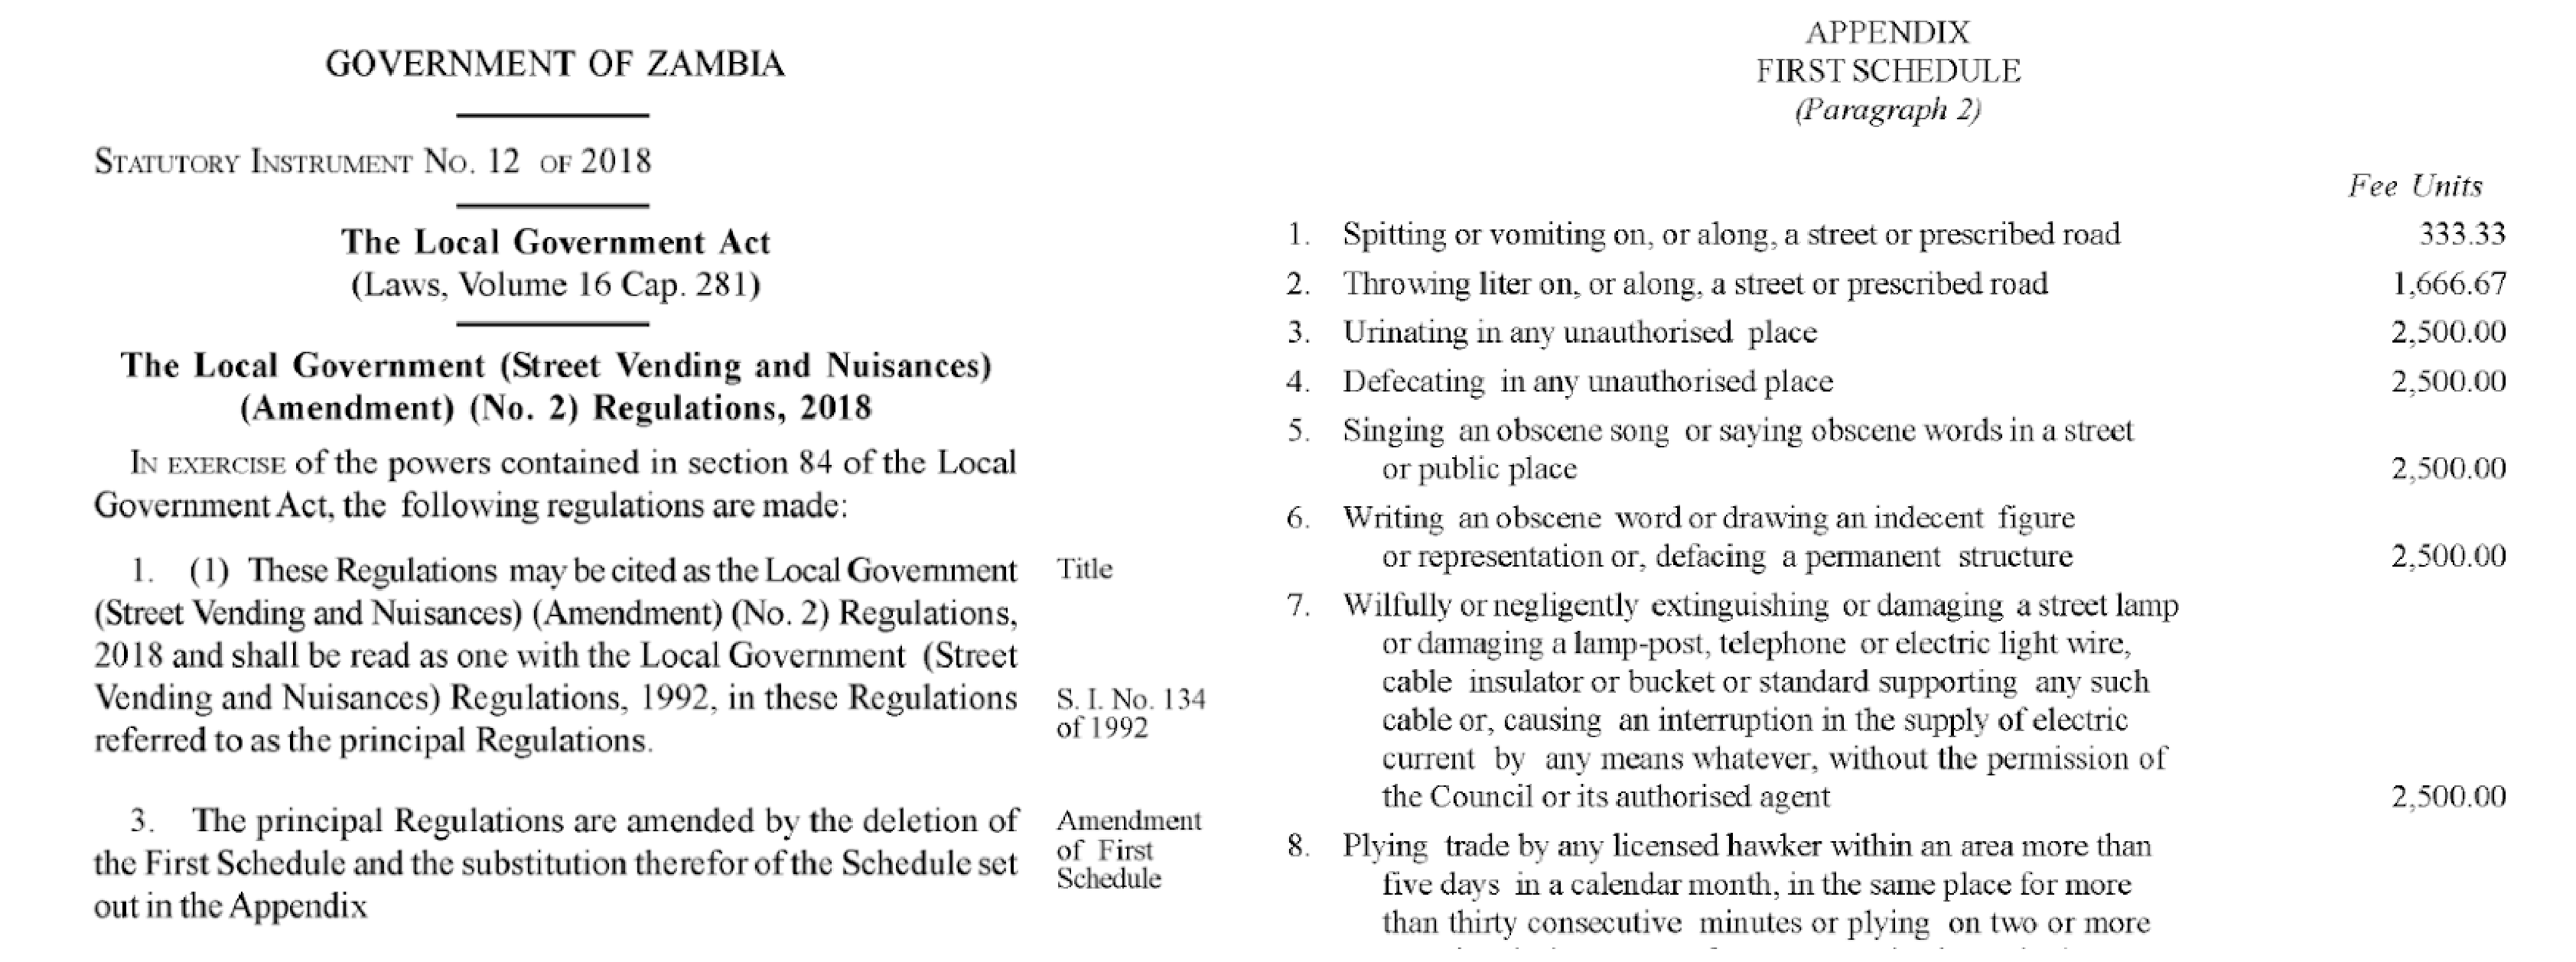
\includegraphics{figures/img-icict24-statutory_instrument12_2018.eps}}
}%
\caption{Statutory Instrument 18 of 2018: Street Vending and Nuisances.}
\label{fig:methodology:understanding_legislation_documents:si18_2018}
\end{figure*}

\subsection{Summarisation Models: Design and Implementation}
\label{sec:methodology:summarisation_models_implementaiton}
The implementation of the NLP summarisation models and pipelines was guided by the Cross-industry Standard Process for Data Mining (CRISP-DM) model \cite{Wirth2000CRISPDM}, with the six (6) phases used as follows:
\begin{enumerate}[label=\textbf{Phase \arabic*.}, leftmargin=*]
    \item Business Understanding---Acts and Bills available on the National Assembly of Zambia Website were analysed to understand the structure of legislative documents
    \item Data Understanding---Data sources were identified, with data extraction conducted on publicly available PDF documents
    \item Data Preparation---Data was pre-processed using common text pre-processing techniques
    \item Modelling---NLP models were implemented in order to summarise legislative documents
    \item Evaluation---Human evaluators were used to determine the most effective summarisation technique---abstractive and extractive summarisation
    \item Deployment---A simple Web-based interface was implemented to comparatively evaluate the two abstractive and extractive summarisations models.
\end{enumerate}

In order to implement effective NLP summarisation models, focus group discussions were held with University of Zambia Law students, in order to understand elements that comprise legislative documents.

Two NLP summarisation models were implemented use two common summarisation techniques: abstractive summarisation and extractive summarisation.

\subsection{Summarisation Models: Comparative Analysis}
\label{sec:methodology:summarisation_models_analysis}
In order to comparatively evaluate the abstractive and extractive summarisation models, a controlled experiment was conducted with human evaluators.

\subsubsection{Task Design}
\label{sec:methodology:summarisation_models_analysis:task_design}
The National Pension Scheme Act No. 1 of 2023\footnote{https://www.parliament.gov.zm/node/11020} was used as input to the two summarisation models and corresponding summaries generated.

\subsubsection{Experimental Design}
\label{sec:methodology:summarisation_models_analysis:experimental_design}
A comparative analysis between the abstractive summarisation model and extractive summarisation model was performed. The study was conducted using a within-subject design, with counterbalancing applied by altering the summarisation models they initially read and rated.

\subsubsection{Procedure}
\label{sec:methodology:summarisation_models_analysis:procedure}
Each participant was required to sign a consent form and subsequently required to read the "National Pension Scheme Act No. 1 of 2023" document and, additionally, the two corresponding summaries. Finally, participants were required to complete a questionnaire design to evaluate the following:
\begin{itemize}
    \item Relevance of each of the two summaries, relative to the original document
    \item Readability ofeach of the two summaries
    \item Prefered summary, when comparing the two generated summaries
\end{itemize}

\section{Results and Discussion}
\label{sec:results_and_discussion}

\subsection{Understanding Legislative Documents}
\label{sec:results_and_discussion:challenges}

The survey gathered responses from 126 undergraduate students, primarily falling within the
18-25 age group, with a mix of participants from various schools and programs of study.
Notably, Humanities and Social Sciences and Veterinary Medicine constituted the majority of
participants. The survey covered students from different study years, with a substantial
representation from Year 2 and Year 3.

The results indicate that a significant portion of participants (98.4\%) have interacted with
Zambian legislative documents, though the frequency varied. The participants provided
diverse responses regarding their overall understanding of legal documents, with the majority
falling within the mid-range on a scale of 1-5.

\begin{figure}%%%%%[htbp]
\fbox{%
\scalebox{0.425}{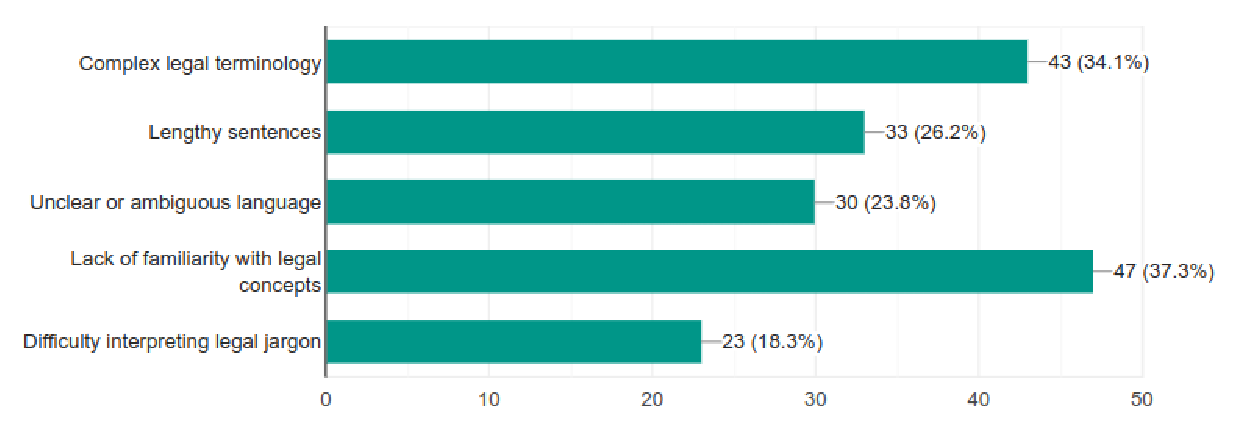
\includegraphics{figures/img-icict24-factors_affecting_legislative_documents.eps}}
}%
\caption{Summmary 2: .}
\label{fig:results_and_discussion:challenges:challenges}
\end{figure}

Participants highlighted various challenges in understanding legal documents, as shown in \Cref{fig:results_and_discussion:challenges:challenges}, including
complex legal terminology, lengthy sentences, unclear or ambiguous language, lack of
familiarity with legal concepts, and difficulty interpreting legal jargon. These challenges
point to potential barriers that may hinder effective comprehension of legislative materials.


\begin{figure}%%%%%[htbp]
\fbox{%
\scalebox{0.415}{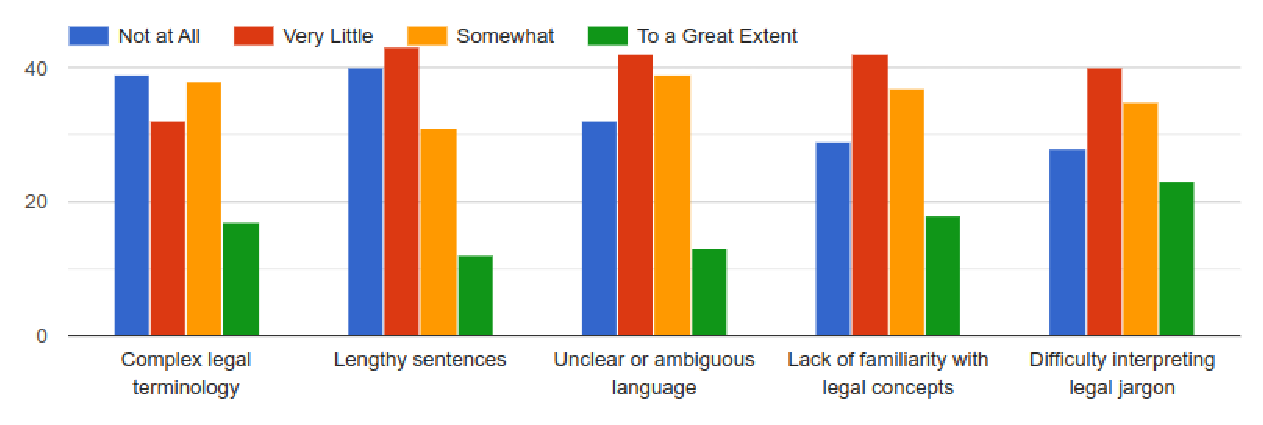
\includegraphics{figures/img-icict24-factors_affecting_legislative_documents_extent.eps}}
}%
\caption{Summmary 2: .}
\label{fig:results_and_discussion:challenges:understanding}
\end{figure}

Factors such as complex legal terminology, lengthy sentences, unclear language, lack of
familiarity with legal concepts, and difficulty interpreting legal jargon were identified as
influencing participants' understanding of legal documents, as shown in \Cref{fig:results_and_discussion:challenges:understanding}. These insights underscore the
need for targeted interventions to address these specific challenges

Participants provided valuable comments and suggestions, emphasising the importance of
brevity and clarity in legal documents. Recommendations included minimising lengthy
sentences, avoiding technical jargon, and making legal documents more accessible.

The survey conducted at the University of Zambia sheds light on the challenges
undergraduate students face in understanding legal documents. The findings indicate a
diverse range of difficulties, encompassing language complexity, sentence structure, and a
lack of familiarity with legal concepts. The insights from this study pave the way for potential
improvements in legal document accessibility and comprehension. The use of automatic
summarization software is suggested as a possible solution to address these challenges,
providing concise and clear summaries of legislative materials.

\subsection{Automatic Summarisation}
\label{sec:results_and_discussion:automatic_summarisation}

\subsubsection{Data Extraction and Pre-processing}
\label{sec:results_and_discussion:automatic_summarisation:data_extraction}
The Python programming language\footnote{https://www.python.org} was used to implement the summarisation models. A two-step process was used to extract data from PDF documents for the purpose of preparing it for subsequent data cleaning. The primary library used for this extraction was PyMuPDF\footnote{https://github.com/pymupdf/PyMuPDF}, specifically the fitz module. This library allows for efficient handling of PDF documents in Python.

In order to use a standardised representation of textual input, case folding was applied to input text.

\subsubsection{Extractive Summarisation Model}
\label{sec:results_and_discussion:automatic_summarisation:extractive}

The evolution of word embedding models progressed with Mikolov et al., who introduced the word2vec model based on skip-grams. This model extended our understanding of word relationships by considering complex
associations, including opposites, tenses, plurals, and phrases. Here, the SpaCy\footnote{https://spacy.io} library plays a
pivotal role in text processing, aiding in the identification and removal of stop words and
punctuation.

\Cref{fig:results_and_discussion:summarisation_models:summary1} illustrates a sample output for the abstractive summarisation model.

\begin{figure}%%%%%[htbp]
\fbox{%
\scalebox{0.65}{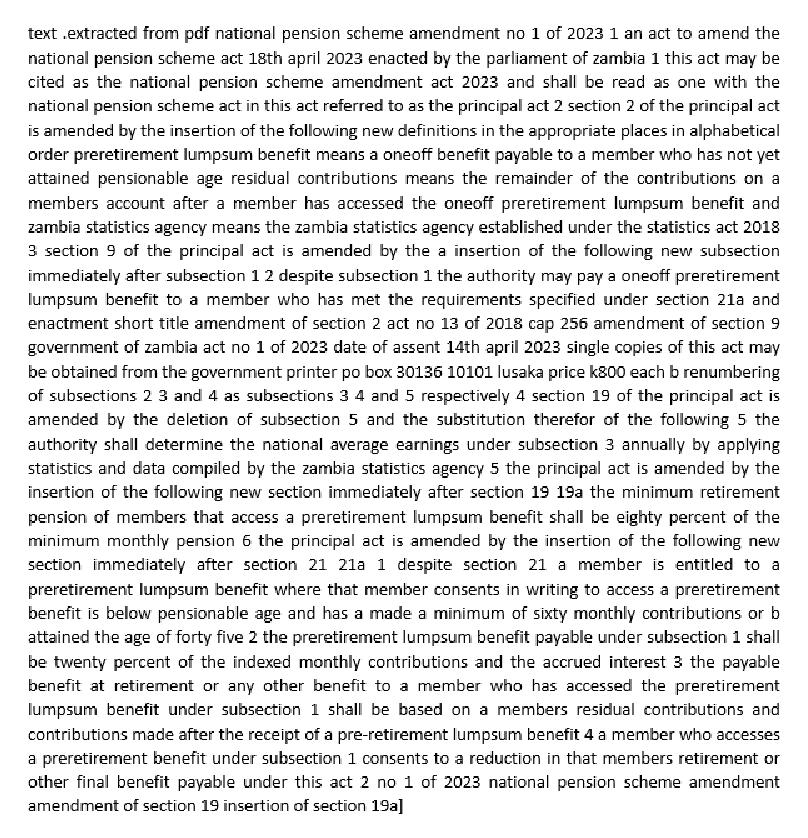
\includegraphics{figures/img-icict24-summary1_output.eps}}
}%
\caption{Summmary 1: Extractive Summarisation.}
\label{fig:results_and_discussion:summarisation_models:summary1}
\end{figure}


\subsubsection{Abstractive Summarisation Model}
\label{sec:results_and_discussion:automatic_summarisation:abstractive}

The abstractive summarisation model was implemented using the BART model from the Hugging Face Transformers library. The
code utilized the "transformers" library to import the necessary components, including the pipeline for text generation, the BART tokenizer, and the BART model for conditional generation. Within the "abstractive\_summarize" function, the pre-trained BART model and tokenizer were loaded using the specified model name "facebook/bart-large-cnn". The input text was then tokenized, and the summary was generated using the BART model. The "generate" method of the model was utilized to produce the summary, with parameters such as maximum and minimum length, length penalty, number of beams, and early stopping specified to control the summarization process. This approach proved to be successful in producing abstractive summaries with the BART model, leveraging its capabilities for text generation and summarization.

\Cref{fig:results_and_discussion:summarisation_models:summary2} illustrates a sample output for the abstractive summarisation model.

\begin{figure}%%%%%[htbp]
\fbox{%
\scalebox{0.345}{\includegraphics{figures/img-icict24-summary2_output.eps}}
}%
\caption{Summmary 2: Abstractive Summarisation.}
\label{fig:results_and_discussion:summarisation_models:summary2}
\end{figure}

By integrating both extractive and abstractive techniques, this project aimed to provide a comprehensive understanding of Zambian legislative materials. The use of diverse Python libraries, including SpaCy for extractive summarization and Transformers BART Model for abstractive summarization, showcased a multifaceted approach to effectively distill and present critical information from lengthy legal documents.


\subsection{Human Comparative Evaluation}
\label{sec:results_and_discussion:human_evaluation}

\begin{figure}%%%%%[htbp]
\fbox{%
\scalebox{0.425}{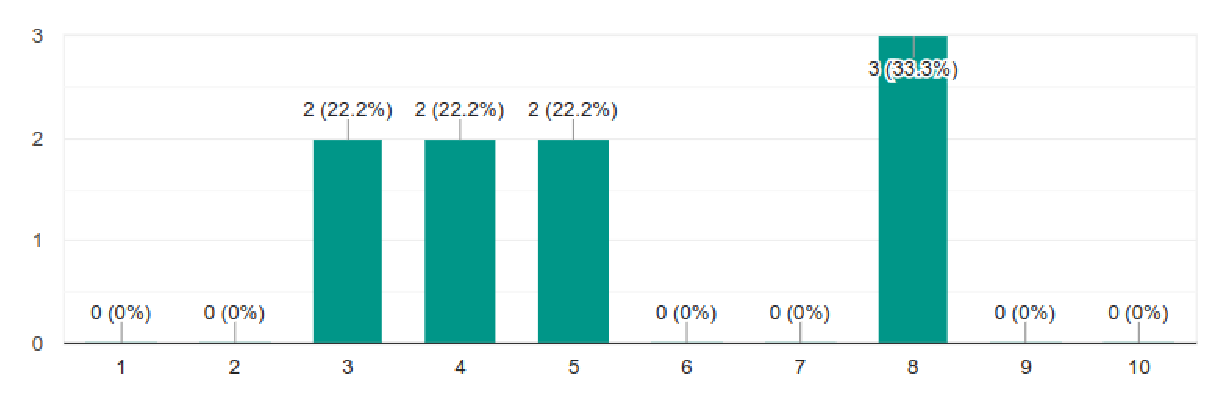
\includegraphics{figures/img-icict24-summary1-relevance.eps}}
}%
\caption{Summmary 1: Relevance.}
\label{fig:results_and_discussion:summarisation_models:summary1_relevance}
\end{figure}

The purpose of this evaluation was to assess the effectiveness of automatic summarization techniques applied to Zambian legislative documents. The participants were asked to read two summaries (Summary 1 - extractive summary, and Summary 2 - abstractive summary) generated from the original legislative document. The evaluation focused on relevance, readability, and preference for conveying information.

\begin{figure}%%%%%[htbp]
\fbox{%
\scalebox{0.425}{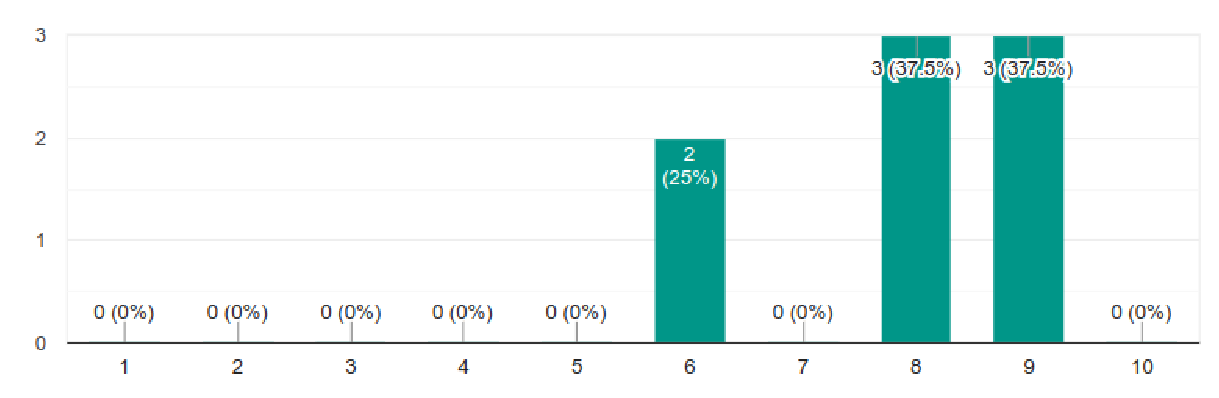
\includegraphics{figures/img-icict24-summary2-relevance.eps}}
}%
\caption{Summmary 2: Relevance.}
\label{fig:results_and_discussion:summarisation_models:summary2_relevance}
\end{figure}

A total of nine participants participated in the comparative evaluation.

The majority of participants who preferred Summary 2 cited its brevity, simplicity, and directness as reasons for their choice. Participants mentioned that Summary 2 was easier to understand and more straightforward. One participant specifically noted that Summary 2 was "straight to the point," enhancing quick comprehension. two participants provided feedback, with one expressing a positive sentiment, stating, "This is good." The other participant did not provide specific comments.

The evaluation indicates a strong preference for Summary 2, the abstractive summary, among participants. While both summaries received similar ratings for relevance and readability, the brevity and directness of Summary 2 seemed to resonate more with participants. The positive feedback aligns with the project's goal of enhancing the accessibility of Zambian legislative information through automatic summarization.

In the relevance evaluation, for the extractive summary (Summary 1), participants rated it between 3 and 8, with none selecting 1, 2, 9, or 10. Similarly, for the abstractive summary (Summary 2), ratings ranged from 3 to 10, with no
participants choosing 1 or 2. In terms of readability, both summaries achieved average scores
around 4.5, reflecting moderate levels of readability. Significantly, the majority of participants (88.9\%) expressed a preference for Summary 2, citing its brevity, simplicity, and directness as reasons for their choice. This preference aligns with the feedback received, where participants highlighted that Summary 2 was easier to understand and more straightforward, with one participant specifically noting that it was "straight to the point," facilitating quick comprehension. Out of the two participants who provided feedback, one expressed a positive sentiment, stating, "This is good," while the other did not provide specific comments.

\begin{figure}%%%%%[htbp]
\fbox{%
\scalebox{0.425}{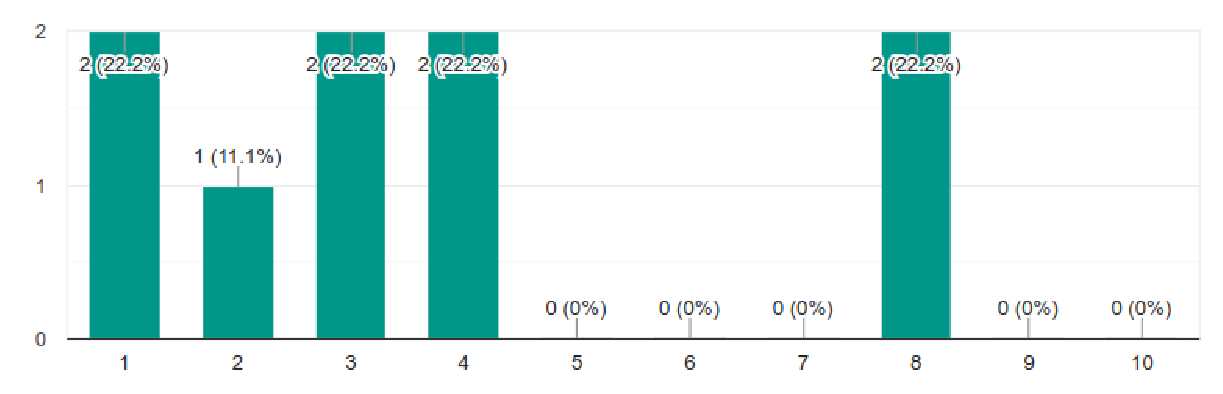
\includegraphics{figures/img-icict24-summary1-readability.eps}}
}%
\caption{Summmary 1: Readability.}
\label{fig:results_and_discussion:summarisation_models:summary1_readability}
\end{figure}


\begin{figure}%%%%%[htbp]
\fbox{%
\scalebox{0.425}{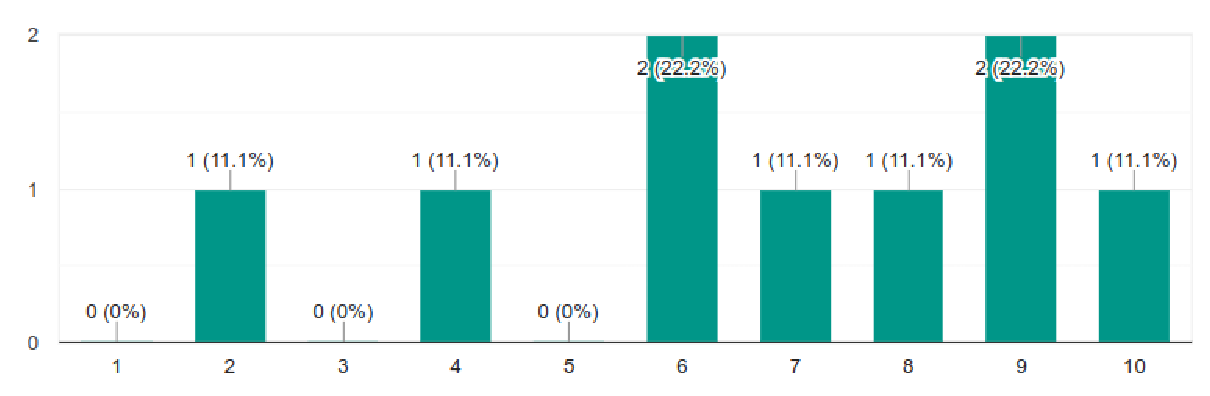
\includegraphics{figures/img-icict24-summary2-readability.eps}}
}%
\caption{Summmary 2: Readability.}
\label{fig:results_and_discussion:summarisation_models:summary2_readability}
\end{figure}

\section{Conclusions and Future Work}
\label{sec:conclusion}
The imperative for automating the summarization of Zambian Legislative Documents becomes evident as it presents an opportunity for citizens to gain quick and enhanced comprehension of lengthy legal documents, including Acts of Parliament. This study aimed at identifying challenges in understanding legislative documents, developing and implementing
an NLP model for automatic summarization, and assessing the model's effectiveness. The evaluation underscores the efficiency of abstractive summarization techniques, particularly noting participant preference in conveying information. These findings offer valuable insights into the strengths and preferences of various summarization approaches, guiding future initiatives to improve the accessibility and understanding of Zambian legislative documents.

% % % % % \section*{References}

\bibliographystyle{IEEEtran}
\bibliography{paper-icict24-automatic_summarisation_of_zambian_legislative_documents}

\end{document}
